\documentclass[a4paper]{article}
\usepackage[a4paper,margin=0mm]{geometry}
\usepackage{fontspec}
\usepackage{unicode-math}
\usepackage{tikz}
\usetikzlibrary{calc}
\usepackage[table]{xcolor}
\usepackage[absolute]{textpos}
\usepackage{enumitem}
\usepackage{array}
\usepackage{multirow}

\setmainfont{Libertinus Serif}
\setsansfont{Libertinus Sans}
\setmathfont{Libertinus Math}

\definecolor{accent}{HTML}{0F6A52}
\definecolor{badge}{HTML}{A9CFC2}
\definecolor{ink}{HTML}{2A2E30}

\setlength{\TPHorizModule}{1mm}
\setlength{\TPVertModule}{1mm}
\setlength{\parindent}{0pt}
\pagestyle{empty}
\binoppenalty=10000 \relpenalty=10000

\newcommand{\LCOL}{16mm}
\newcommand{\RCOL}{111mm}
\newcommand{\COLW}{83mm}

\newcommand{\topicheader}[2]{%
\begin{textblock*}{194mm}(16mm,10mm)
\begin{tikzpicture}
\node[fill=accent,text=white,font=\sffamily\bfseries\fontsize{13}{13}\selectfont,
      minimum width=9mm,minimum height=9mm,inner sep=0pt] at (4.5mm,-4.5mm) {#1};
\node[font=\sffamily\bfseries\fontsize{15}{16}\selectfont,text=ink,anchor=west] at (12mm,-4.5mm) {#2};
\end{tikzpicture}
\end{textblock*}
\begin{textblock*}{194mm}(16mm,22.5mm)

\begin{tikzpicture}
\fill[accent] (0,0) rectangle (194mm,0.5mm);
\end{tikzpicture}
\end{textblock*}
}

\newcommand{\pagefooter}[1]{%
\begin{textblock*}{194mm}(8mm,286.41mm)
  
\begin{tikzpicture}
    \fill[accent] (0,0) rectangle (194mm,0.6mm);
  \end{tikzpicture}
\end{textblock*}
\begin{textblock*}{63.59mm}(8mm,288.27mm)
  {\sffamily\bfseries\color{accent}\fontsize{13}{16}\selectfont SAT 1200+}
\end{textblock*}
\begin{textblock*}{10mm}(188mm,288.27mm)
  \centering{\sffamily\color{accent}\fontsize{14}{16}\selectfont #1}
\end{textblock*}
}

\newcommand{\colrule}[2]{%
\begin{textblock*}{1mm}(105mm,#1mm)
\begin{tikzpicture}
\draw[black!65,line width=0.5pt] (0,0) -- (0,#2mm);
\end{tikzpicture}
\end{textblock*}
}

% Page kicker: left = module line, right = question range
\newcommand{\pagekicker}[2]{%
\begin{textblock*}{194mm}(16mm,25.2mm)
{\sffamily\bfseries\fontsize{10.5}{12}\selectfont\color{accent}#1}\hfill{\sffamily\fontsize{10}{12}\selectfont\color{black!70}#2}
\end{textblock*}
}

\setlength{\fboxsep}{1.4pt}
\setlength{\fboxrule}{0.5pt}
\newcommand{\pnum}[1]{\fcolorbox{ink}{white}{\sffamily\bfseries\fontsize{8}{8}\selectfont #1}~}

% centered display line inside a stem
\newcommand{\dsp}[1]{\par\vspace{1.4mm}\centerline{#1}\vspace{1.8mm}}

% student-produced response box
\newcommand{\gridbox}{%
\par\vspace{3mm}\noindent

\begin{tikzpicture}
\node[anchor=south west,font=\sffamily\bfseries\fontsize{7.5}{9}\selectfont,text=accent,inner sep=0pt] at (0,0.3mm) {STUDENT-PRODUCED RESPONSE};
\draw[ink,line width=0.7pt] (0,-9.5mm) rectangle (40mm,-0.8mm);
\node[anchor=west,font=\sffamily\fontsize{7.5}{9}\selectfont,text=black!55,inner sep=0pt] at (43mm,-5.2mm) {Write your answer in the box.};
\end{tikzpicture}\par}

\arrayrulecolor{accent}
\setlength{\arrayrulewidth}{0.7pt}
\renewcommand{\arraystretch}{1.35}

\newcommand{\figwrap}[1]{\par\vspace{2.5mm}\centerline{{\arrayrulecolor{ink}\setlength{\arrayrulewidth}{0.5pt}\renewcommand{\arraystretch}{1.3}#1}}\vspace{0.5mm}}

\begin{document}

% ================= PAGE 1: Mock Test 2 -- instructions + geometry reference sheet =================
\topicheader{2}{Mock Test 2}
\pagefooter{1}
\mbox{}%

\newcommand{\cardhead}[1]{{\sffamily\bfseries\color{accent}\fontsize{11.5}{14}\selectfont #1}\par\vspace{0.6mm}%
{\color{accent}\rule{\linewidth}{0.5pt}}\par\vspace{1.6mm}}
\newcommand{\bul}{\item[\textcolor{accent}{\rule[0.2mm]{1.5mm}{1.5mm}}]}

\begin{textblock*}{194mm}(16mm,28mm)
{\sffamily\bfseries\color{accent}\fontsize{26}{28}\selectfont Mock Test 2\par}
\vspace{1mm}
{\sffamily\color{ink}\fontsize{11}{14}\selectfont Full-length digital SAT Math practice \;\textperiodcentered\; 2 modules $\times$ 22 questions $\times$ 35 minutes\par}
\end{textblock*}

\begin{textblock*}{\COLW}(\LCOL,53mm)
{\fontsize{9.4}{12.2}\selectfont
\cardhead{How this test works}
\renewcommand{\arraystretch}{1.3}\setlength{\tabcolsep}{4pt}
\noindent\begin{tabular}{|>{\raggedright\arraybackslash}p{20mm}|>{\centering\arraybackslash}p{15mm}|>{\centering\arraybackslash}p{13mm}|>{\centering\arraybackslash}p{19mm}|}
\hline
\rowcolor{badge!55}\textbf{Module} & \textbf{Questions} & \textbf{Time} & \textbf{Calculator}\\\hline
Module 1 & 22 & 35 min & allowed\\\hline
Module 2 & 22 & 35 min & allowed\\\hline
\end{tabular}\par\vspace{2.2mm}
\begin{itemize}[leftmargin=5mm,itemsep=1.2mm,topsep=0mm,parsep=0mm]
\bul Time each module separately: 35 minutes, not a minute more. Rest for 5--10 minutes between the two modules.
\bul Use a calculator (the built-in Desmos graphing calculator or any approved calculator) on both modules.
\bul Module 1 is a standard mix of easy, medium and hard questions. Module 2 is the \emph{harder route} you reach by doing well on Module 1.
\bul Answer every question. There is no penalty for a wrong answer.
\bul Unless a problem says otherwise, all numbers are real, a function's domain is every real number for which it is defined, and figures are not necessarily drawn to scale.
\bul Do not look at any answers while you work. When you finish both modules, score yourself with the \textbf{Answer Sheets} section at the end of this book.
\end{itemize}
}
\end{textblock*}

\begin{textblock*}{\COLW}(\RCOL,53mm)
{\fontsize{9.4}{12.2}\selectfont
\cardhead{Student-produced responses (grid-ins)}
Some questions have no answer choices. Work out the answer and write it in the answer box (on the real test you type it in).
\begin{itemize}[leftmargin=5mm,itemsep=1.2mm,topsep=1.6mm,parsep=0mm]
\bul You may give an integer, a decimal, or a fraction. For one answer, $9/2$ and $4.5$ are both correct.
\bul Never enter a mixed number: write $7/2$ or $3.5$, not $3\,1/2$ (it would be read as $31/2$).
\bul Do not enter symbols or units such as \$, \%, or $\pi$. Enter the number only.
\bul An answer may use at most 5 characters (6 if it is negative), counting the slash and the decimal point.
\bul If an answer is a repeating decimal, enter it as a fraction such as $2/3$, or fill all the digits that fit: $0.6666$ or $0.6667$.
\bul If you find more than one correct answer, enter only one of them.
\end{itemize}
\vspace{1.2mm}
\noindent\fcolorbox{accent}{badge!25}{\parbox{\dimexpr\linewidth-2\fboxsep-2\fboxrule}{\centering\sffamily\fontsize{8.5}{11}\selectfont
\textbf{Example.} Answer $4\tfrac12$ \;$\rightarrow$\; enter \textbf{9/2} or \textbf{4.5}\par}}
\par\vspace{3mm}
\noindent{\sffamily\bfseries\color{accent}Pacing.}\ Q1--15: about 18 min. Q16--22: about 17 min. Keep the last 2--3 min for flagged questions and every blank grid-in (a blank is a guaranteed zero).
}
\end{textblock*}

% ---- Geometry reference sheet (full width card) ----
\begin{textblock*}{178mm}(16mm,156mm)
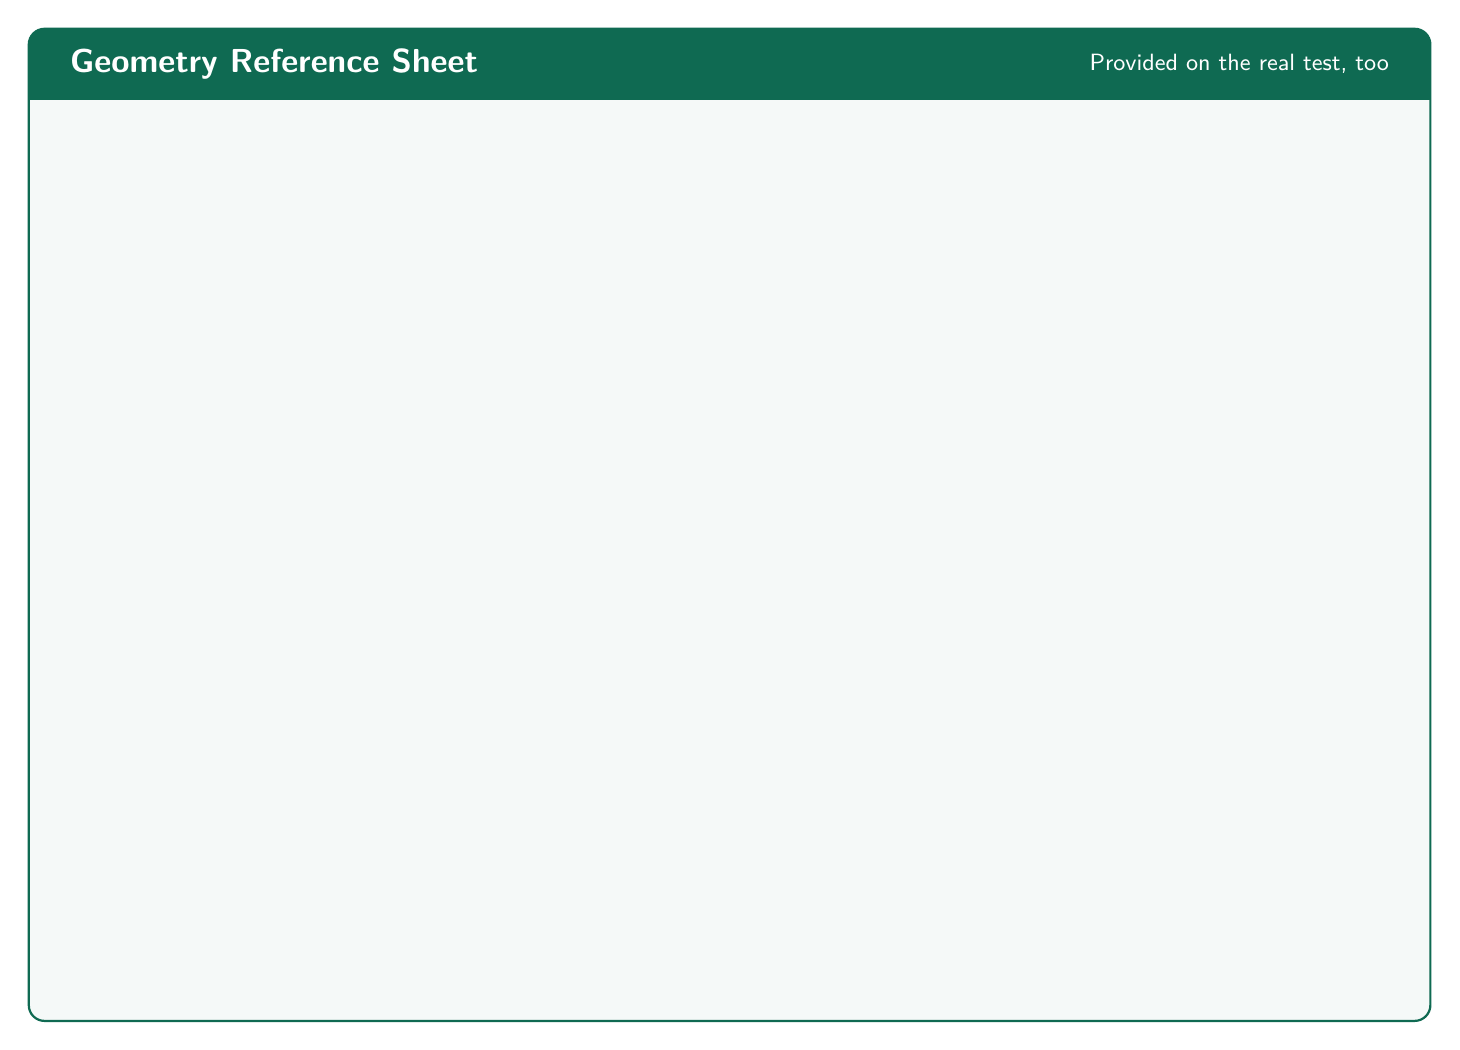
\begin{tikzpicture}
\draw[accent,line width=0.8pt,rounded corners=2mm,fill=badge!12] (0,0) rectangle (178mm,-126mm);
\fill[accent,rounded corners=2mm] (0,0) rectangle (178mm,-9mm);
\fill[accent] (0,-5mm) rectangle (178mm,-9mm);
\node[anchor=west,text=white,font=\sffamily\bfseries\fontsize{12}{14}\selectfont] at (4mm,-4.5mm) {Geometry Reference Sheet};
\node[anchor=east,text=white,font=\sffamily\fontsize{8.5}{10}\selectfont] at (174mm,-4.5mm) {Provided on the real test, too};
\end{tikzpicture}
\end{textblock*}

\newcommand{\refcell}[3]{\begin{textblock*}{42mm}(#1mm,#2mm)\begin{minipage}[t][36mm][t]{42mm}\centering #3\end{minipage}\end{textblock*}}
\newcommand{\refin}[2]{\parbox[b][26mm][b]{42mm}{\centering #1}\par\vspace{1.6mm}{\fontsize{9.6}{11.5}\selectfont #2}}
\tikzset{rf/.style={ink,line width=0.65pt},lb/.style={font=\fontsize{8.5}{9.5}\selectfont,inner sep=1.2pt}}

% ---------- row 1
\refcell{18}{167}{\refin{\begin{tikzpicture}[scale=1.25]
\draw[rf] (0,0) circle (9mm); \draw[rf] (0,0)--(9mm,0); \fill[ink] (0,0) circle (0.7pt);
\node[lb,above] at (4.5mm,0) {$r$};
\end{tikzpicture}}{Circle\\$A=\pi r^{2}$,\; $C=2\pi r$}}
\refcell{62}{167}{\refin{\begin{tikzpicture}[scale=1.25]
\draw[rf] (0,0) rectangle (22mm,12mm);
\node[lb,below] at (11mm,0) {$\ell$}; \node[lb,right] at (22mm,6mm) {$w$};
\end{tikzpicture}}{Rectangle\\$A=\ell w$}}
\refcell{106}{167}{\refin{\begin{tikzpicture}[scale=1.25]
\draw[rf] (0,0)--(22mm,0)--(7mm,13mm)--cycle;
\draw[rf,dashed] (7mm,0)--(7mm,13mm);
\draw[rf] (7mm,0)++(0,1.8mm)--++(1.8mm,0)--++(0,-1.8mm);
\node[lb,below] at (11mm,0) {$b$}; \node[lb,left] at (7mm,6.5mm) {$h$};
\end{tikzpicture}}{Triangle\\$A=\tfrac12 bh$}}
\refcell{150}{167}{\refin{\begin{tikzpicture}[scale=1.25]
\draw[rf] (0,0)--(18mm,0)--(0,12mm)--cycle;
\draw[rf] (0,1.8mm)--(1.8mm,1.8mm)--(1.8mm,0);
\node[lb,below] at (9mm,0) {$a$}; \node[lb,left] at (0,6mm) {$b$}; \node[lb,above right] at (9mm,6mm) {$c$};
\end{tikzpicture}}{Right triangle\\$c^{2}=a^{2}+b^{2}$}}

% ---------- row 2
\refcell{18}{204}{\refin{\begin{tikzpicture}[scale=1.25]
\draw[rf] (0,0)--(19.053mm,0)--(0,11mm)--cycle;
\draw[rf] (0,1.8mm)--(1.8mm,1.8mm)--(1.8mm,0);
\node[lb,below] at (9.5mm,0) {$x\sqrt3$}; \node[lb,left] at (0,5.5mm) {$x$}; \node[lb,above right] at (9.5mm,5.5mm) {$2x$};
\node[lb] at (14.6mm,1.9mm) {\fontsize{6.5}{7}\selectfont$30^\circ$}; \node[lb] at (3.2mm,8.2mm) {\fontsize{6.5}{7}\selectfont$60^\circ$};
\end{tikzpicture}}{$30^\circ$--$60^\circ$--$90^\circ$ triangle}}
\refcell{62}{204}{\refin{\begin{tikzpicture}[scale=1.25]
\draw[rf] (0,0)--(10mm,0)--(0,10mm)--cycle;
\draw[rf] (0,1.8mm)--(1.8mm,1.8mm)--(1.8mm,0);
\node[lb,below] at (5mm,0) {$s$}; \node[lb,left] at (0,5mm) {$s$}; \node[lb,above right] at (5mm,5mm) {$s\sqrt2$};
\end{tikzpicture}}{$45^\circ$--$45^\circ$--$90^\circ$ triangle}}
\refcell{106}{204}{\refin{\begin{tikzpicture}[scale=1.2]
\draw[rf] (0,0) rectangle (16mm,9mm);
\draw[rf] (16mm,9mm)--(22mm,13mm)--(6mm,13mm)--(0,9mm);
\draw[rf] (16mm,0)--(22mm,4mm)--(22mm,13mm);
\draw[rf,dashed] (6mm,13mm)--(6mm,4mm)--(22mm,4mm); \draw[rf,dashed] (0,0)--(6mm,4mm);
\node[lb,below] at (8mm,0) {$\ell$}; \node[lb,right] at (22mm,8.5mm) {$h$}; \node[lb,below right] at (19mm,2mm) {$w$};
\end{tikzpicture}}{Rectangular solid\\$V=\ell wh$}}
\refcell{150}{204}{\refin{\begin{tikzpicture}[scale=1.2]
\draw[rf] (0,2.2mm) ellipse (7mm and 2.2mm);
\draw[rf] (-7mm,2.2mm)--(-7mm,14mm); \draw[rf] (7mm,2.2mm)--(7mm,14mm);
\draw[rf] (0,14mm) ellipse (7mm and 2.2mm);
\draw[rf,dashed] (0,14mm)--(7mm,14mm); \fill[ink] (0,14mm) circle (0.6pt);
\node[lb,above] at (3.5mm,14mm) {$r$}; \node[lb,right] at (7mm,8mm) {$h$};
\end{tikzpicture}}{Right circular cylinder\\$V=\pi r^{2}h$}}

% ---------- row 3
\refcell{18}{241}{\refin{\begin{tikzpicture}[scale=1.15]
\draw[rf] (0,0) circle (10mm);
\draw[rf] (-10mm,0) arc (180:360:10mm and 2.8mm); \draw[rf,dashed] (-10mm,0) arc (180:0:10mm and 2.8mm);
\draw[rf] (0,0)--(10mm,0); \fill[ink] (0,0) circle (0.7pt); \node[lb,above] at (5mm,0) {$r$};
\end{tikzpicture}}{Sphere\\$V=\tfrac43\pi r^{3}$}}
\refcell{62}{241}{\refin{\begin{tikzpicture}[scale=1.2]
\draw[rf] (0,2.2mm) ellipse (7mm and 2.2mm);
\draw[rf] (-7mm,2.2mm)--(0,16mm)--(7mm,2.2mm);
\draw[rf,dashed] (0,16mm)--(0,2.2mm); \draw[rf,dashed] (0,2.2mm)--(7mm,2.2mm);
\fill[ink] (0,2.2mm) circle (0.6pt);
\node[lb,left] at (0,9.5mm) {$h$}; \node[lb,above] at (3.5mm,2.2mm) {$r$};
\end{tikzpicture}}{Right circular cone\\$V=\tfrac13\pi r^{2}h$}}
\refcell{106}{241}{\refin{\begin{tikzpicture}[scale=1.2]
\draw[rf] (0,0)--(16mm,0)--(22mm,4mm); \draw[rf] (0,0)--(10mm,15mm)--(16mm,0); \draw[rf] (10mm,15mm)--(22mm,4mm);
\draw[rf,dashed] (0,0)--(6mm,4mm)--(22mm,4mm); \draw[rf,dashed] (6mm,4mm)--(10mm,15mm);
\node[lb,below] at (8mm,0) {$\ell$}; \node[lb,below right] at (19mm,2mm) {$w$}; \node[lb,left] at (10mm,9.5mm) {$h$};
\end{tikzpicture}}{Rectangular pyramid\\$V=\tfrac13\ell wh$}}
\begin{textblock*}{40mm}(151mm,247mm)
{\fontsize{9.2}{12}\selectfont\raggedright
\textcolor{accent}{\rule[0.3mm]{1.6mm}{1.6mm}}\; A circle has 360 degrees of arc.\par\vspace{1.2mm}
\textcolor{accent}{\rule[0.3mm]{1.6mm}{1.6mm}}\; The angles of a triangle add up to 180 degrees.\par\vspace{1.2mm}
\textcolor{accent}{\rule[0.3mm]{1.6mm}{1.6mm}}\; $r$ radius, $\ell$ length, $w$ width, $b$ base, $h$ height.\par}
\end{textblock*}

\clearpage

% ===== Module 1, page 1 =====
\topicheader{2}{Mock Test 2}
\pagefooter{2}
\colrule{34}{236}
\mbox{}%
\pagekicker{Mock 2 \textperiodcentered{} Module 1 \textperiodcentered{} 22 questions \textperiodcentered{} 35 minutes}{Questions 1--8}
\begin{textblock*}{\COLW}(\LCOL,34mm)
{\fontsize{10.4}{13.4}\selectfont
\parbox[t][233mm][t]{\COLW}{%
\noindent\pnum{1} If $6a+5=41$, what is the value of $a$?\par\vspace{2.2mm}
\hspace*{7mm}(A)\ $6$\\[1.8mm]
\hspace*{7mm}(B)\ $7$\\[1.8mm]
\hspace*{7mm}(C)\ $\dfrac{23}{3}$\\[1.8mm]
\hspace*{7mm}(D)\ $36$
\vfill

\noindent\pnum{2} The function $g$ is defined by $g(t)=5\cdot2^{t}$. What is the value of $g(3)$?\par\vspace{2.2mm}
\hspace*{7mm}(A)\ $30$\\[1.8mm]
\hspace*{7mm}(B)\ $40$\\[1.8mm]
\hspace*{7mm}(C)\ $125$\\[1.8mm]
\hspace*{7mm}(D)\ $1000$
\vfill

\noindent\pnum{3} A lab keeps 250 mice, and 36\% of them are female. How many of the mice are female?\par\vspace{2.2mm}
\hspace*{7mm}(A)\ $25$\\[1.8mm]
\hspace*{7mm}(B)\ $36$\\[1.8mm]
\hspace*{7mm}(C)\ $90$\\[1.8mm]
\hspace*{7mm}(D)\ $160$
\vfill

\noindent\pnum{4} Two angles are supplementary. One angle measures $5x^{\circ}$ and the other measures $(x+30)^{\circ}$. What is the measure, in degrees, of the larger angle?\gridbox
\vfill}}
\end{textblock*}
\begin{textblock*}{\COLW}(\RCOL,34mm)
{\fontsize{10.4}{13.4}\selectfont
\parbox[t][233mm][t]{\COLW}{%
\noindent\pnum{5} A taxi company charges a flat fee of \$4 plus \$2.50 for each mile traveled. Dana's fare for one ride was \$29. How many miles did Dana ride?\par\vspace{2.2mm}
\hspace*{7mm}(A)\ $10$\\[1.8mm]
\hspace*{7mm}(B)\ $11.6$\\[1.8mm]
\hspace*{7mm}(C)\ $13.2$\\[1.8mm]
\hspace*{7mm}(D)\ $25$
\vfill

\noindent\pnum{6} Which of the following is equivalent to $(2x+3)(x-5)$?\par\vspace{2.2mm}
\hspace*{7mm}(A)\ $2x^2-13x-15$\\[1.8mm]
\hspace*{7mm}(B)\ $2x^2-7x+15$\\[1.8mm]
\hspace*{7mm}(C)\ $2x^2+7x-15$\\[1.8mm]
\hspace*{7mm}(D)\ $2x^2-7x-15$
\vfill

\noindent\pnum{7} In the $xy$-plane, the graph of $3x+4y=24$ crosses the $x$-axis at the point $(a,0)$. What is the value of $a$?\gridbox
\vfill

\noindent\pnum{8} The function $f$ is defined by $f(x)=(x-4)^2+9$. What is the minimum value of $f$?\par\vspace{2.2mm}
\hspace*{7mm}(A)\ $-4$\\[1.8mm]
\hspace*{7mm}(B)\ $4$\\[1.8mm]
\hspace*{7mm}(C)\ $9$\\[1.8mm]
\hspace*{7mm}(D)\ $25$
\vfill}}
\end{textblock*}
\clearpage

% ===== Module 1, page 2 =====
\topicheader{2}{Mock Test 2}
\pagefooter{3}
\colrule{34}{236}
\mbox{}%
\pagekicker{Mock 2 \textperiodcentered{} Module 1 \textperiodcentered{} 22 questions \textperiodcentered{} 35 minutes}{Questions 9--16}
\begin{textblock*}{\COLW}(\LCOL,34mm)
{\fontsize{10.4}{13.4}\selectfont
\parbox[t][233mm][t]{\COLW}{%
\noindent\pnum{9} At a regional swim meet, a random sample of 150 of the 2,500 swimmers was selected, and 36 of the swimmers in the sample had qualified for the final round. Based on the sample, which of the following is the best estimate of the number of swimmers at the meet who qualified for the final round?\par\vspace{2.2mm}
\hspace*{7mm}(A)\ $60$\\[1.8mm]
\hspace*{7mm}(B)\ $600$\\[1.8mm]
\hspace*{7mm}(C)\ $2464$\\[1.8mm]
\hspace*{7mm}(D)\ $10417$
\vfill

\noindent\pnum{10} A reservoir is being drained. The equation $V=420-56t$ gives the volume $V$, in thousands of cubic meters, of water in the reservoir $t$ hours after draining began. Which of the following is the best interpretation of the point $(5,140)$ on the graph of this equation in the $tV$-plane?\par\vspace{2.2mm}
\hspace*{7mm}(A)\ After 5 hours, 140 thousand cubic meters of water have been drained.\\[1.8mm]
\hspace*{7mm}(B)\ After 140 hours, the reservoir holds 5 thousand cubic meters of water.\\[1.8mm]
\hspace*{7mm}(C)\ During the fifth hour, 140 thousand cubic meters of water are drained.\\[1.8mm]
\hspace*{7mm}(D)\ After 5 hours, the reservoir holds 140 thousand cubic meters of water.
\vfill

\noindent\pnum{11} The graphs of $2x+y=11$ and $x-3y=-12$ intersect at the point $(p,q)$ in the $xy$-plane. What is the value of $pq$?\gridbox
\vfill

\noindent\pnum{12} The function $f$ is defined by $f(x)=x^2+bx+12$, where $b$ is a constant. If $f(3)=0$, what is the value of $f(-1)$?\par\vspace{2.2mm}
\hspace*{7mm}(A)\ $30$\\[1.8mm]
\hspace*{7mm}(B)\ $20$\\[1.8mm]
\hspace*{7mm}(C)\ $12$\\[1.8mm]
\hspace*{7mm}(D)\ $6$
\vfill}}
\end{textblock*}
\begin{textblock*}{\COLW}(\RCOL,34mm)
{\fontsize{10.4}{13.4}\selectfont
\parbox[t][233mm][t]{\COLW}{%
\noindent\pnum{13} In the $xy$-plane, the points $P(-1,2)$ and $Q(5,10)$ are the endpoints of a diameter of a circle. What is the area of the circle?\par\vspace{2.2mm}
\hspace*{7mm}(A)\ $5\pi$\\[1.8mm]
\hspace*{7mm}(B)\ $10\pi$\\[1.8mm]
\hspace*{7mm}(C)\ $25\pi$\\[1.8mm]
\hspace*{7mm}(D)\ $100\pi$
\vfill

\noindent\pnum{14} The table shows the number of goals a soccer team scored in each of its 20 games this season. What was the mean number of goals the team scored per game?\figwrap{\begin{tabular}{|l|c|c|c|c|c|}
\hline
Goals in a game & 0 & 1 & 2 & 3 & 4\\\hline
Number of games & 3 & 5 & 6 & 4 & 2\\\hline
\end{tabular}}\gridbox
\vfill

\noindent\pnum{15} Let $A=2x^2-3x+1$ and $B=x^2+4x-5$. Which of the following is equivalent to $A-2B$?\par\vspace{2.2mm}
\hspace*{7mm}(A)\ $-11x+11$\\[1.8mm]
\hspace*{7mm}(B)\ $-11x-9$\\[1.8mm]
\hspace*{7mm}(C)\ $x^2-7x+6$\\[1.8mm]
\hspace*{7mm}(D)\ $4x^2+5x-9$
\vfill

\noindent\pnum{16} A cyclist rode a total of 50 kilometers in 2.75 hours. Part of the ride was at a constant speed of 20 kilometers per hour and the rest was at a constant speed of 15 kilometers per hour. How many kilometers did the cyclist ride at 20 kilometers per hour?\par\vspace{2.2mm}
\hspace*{7mm}(A)\ $15$\\[1.8mm]
\hspace*{7mm}(B)\ $25$\\[1.8mm]
\hspace*{7mm}(C)\ $35$\\[1.8mm]
\hspace*{7mm}(D)\ $50$
\vfill}}
\end{textblock*}
\clearpage

% ===== Module 1, page 3 =====
\topicheader{2}{Mock Test 2}
\pagefooter{4}
\colrule{34}{236}
\mbox{}%
\pagekicker{Mock 2 \textperiodcentered{} Module 1 \textperiodcentered{} 22 questions \textperiodcentered{} 35 minutes}{Questions 17--22}
\begin{textblock*}{\COLW}(\LCOL,34mm)
{\fontsize{10.4}{13.4}\selectfont
\parbox[t][233mm][t]{\COLW}{%
\noindent\pnum{17} What is the solution to the equation below?\dsp{$\dfrac{2}{3}(x-6)=\dfrac{x+2}{2}$}\gridbox
\vfill

\noindent\pnum{18} A ball is thrown upward from the top of a cliff. The height $h$, in meters, of the ball above the ground $t$ seconds after it is thrown is given by $h(t)=-5t^2+20t+60$. At what time $t$, in seconds, does the ball hit the ground?\par\vspace{2.2mm}
\hspace*{7mm}(A)\ $-2$\\[1.8mm]
\hspace*{7mm}(B)\ $2$\\[1.8mm]
\hspace*{7mm}(C)\ $4$\\[1.8mm]
\hspace*{7mm}(D)\ $6$
\vfill

\noindent\pnum{19} The expression $x-2$ is a factor of $p(x)=x^3-5x^2+kx+6$, where $k$ is a constant. What is the value of $k$?\par\vspace{2.2mm}
\hspace*{7mm}(A)\ $3$\\[1.8mm]
\hspace*{7mm}(B)\ $6$\\[1.8mm]
\hspace*{7mm}(C)\ $11$\\[1.8mm]
\hspace*{7mm}(D)\ $17$
\vfill}}
\end{textblock*}
\begin{textblock*}{\COLW}(\RCOL,34mm)
{\fontsize{10.4}{13.4}\selectfont
\parbox[t][233mm][t]{\COLW}{%
\noindent\pnum{20} A motorboat travels 24 kilometers upstream and then returns the same 24 kilometers downstream. The speed of the river's current is 2 kilometers per hour, and the round trip takes 5 hours. What is the boat's speed downstream, in kilometers per hour?\par\vspace{2.2mm}
\hspace*{7mm}(A)\ $5$\\[1.8mm]
\hspace*{7mm}(B)\ $8$\\[1.8mm]
\hspace*{7mm}(C)\ $10$\\[1.8mm]
\hspace*{7mm}(D)\ $12$
\vfill

\noindent\pnum{21} In the figure, triangle $ABC$ has a right angle at $C$. Point $D$ lies on $\overline{AB}$ so that $\overline{CD}$ is perpendicular to $\overline{AB}$. If $AD=4$ and $DB=9$, what is the area of triangle $ABC$?\figwrap{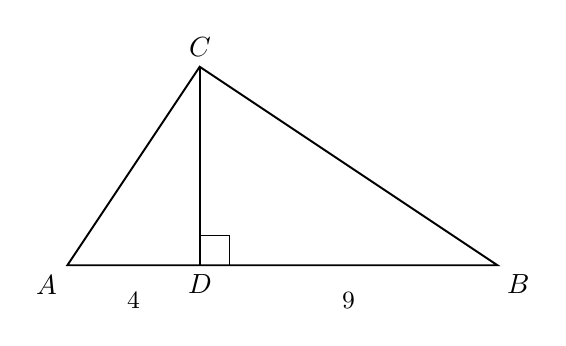
\begin{tikzpicture}[scale=0.42]
\coordinate (A) at (0,0); \coordinate (B) at (13,0); \coordinate (C) at (4,6); \coordinate (D) at (4,0);
\draw[line width=0.7pt] (A)--(B)--(C)--cycle;
\draw[line width=0.7pt] (C)--(D);
\draw[line width=0.5pt] (4,0.9)--(4.9,0.9)--(4.9,0);
\node[below left] at (A) {$A$}; \node[below right] at (B) {$B$}; \node[above] at (C) {$C$}; \node[below] at (D) {$D$};
\node[below,font=\small] at (2,-0.5) {4}; \node[below,font=\small] at (8.5,-0.5) {9};
\end{tikzpicture}}\gridbox
\vfill

\noindent\pnum{22} In the $xy$-plane, line $\ell$ has equation $2x+y=14$, and line $m$ passes through the points $(2,0)$ and $(5,9)$. Lines $\ell$ and $m$ and the $x$-axis form a triangle. What is the area of the triangle?\par\vspace{2.2mm}
\hspace*{7mm}(A)\ $7.5$\\[1.8mm]
\hspace*{7mm}(B)\ $15$\\[1.8mm]
\hspace*{7mm}(C)\ $21$\\[1.8mm]
\hspace*{7mm}(D)\ $30$
\vfill}}
\end{textblock*}
\clearpage

% ===== Module 2, page 1 =====
\topicheader{2}{Mock Test 2}
\pagefooter{5}
\colrule{34}{236}
\mbox{}%
\pagekicker{Mock 2 \textperiodcentered{} Module 2 \textperiodcentered{} 22 questions \textperiodcentered{} 35 minutes}{Questions 1--8}
\begin{textblock*}{\COLW}(\LCOL,34mm)
{\fontsize{10.4}{13.4}\selectfont
\parbox[t][233mm][t]{\COLW}{%
\noindent\pnum{1} If $\frac{2}{5}x=14$, what is the value of $x$?\par\vspace{2.2mm}
\hspace*{7mm}(A)\ $5.6$\\[1.8mm]
\hspace*{7mm}(B)\ $28$\\[1.8mm]
\hspace*{7mm}(C)\ $35$\\[1.8mm]
\hspace*{7mm}(D)\ $70$
\vfill

\noindent\pnum{2} If $3^{x+1}=81$, what is the value of $x$?\par\vspace{2.2mm}
\hspace*{7mm}(A)\ $3$\\[1.8mm]
\hspace*{7mm}(B)\ $4$\\[1.8mm]
\hspace*{7mm}(C)\ $26$\\[1.8mm]
\hspace*{7mm}(D)\ $27$
\vfill

\noindent\pnum{3} On a map, 1 centimeter represents 4.5 kilometers. Two towns are 3.2 centimeters apart on the map. A bus travels the straight-line distance between the towns at a constant speed of 72 kilometers per hour. How many minutes does the trip take?\par\vspace{2.2mm}
\hspace*{7mm}(A)\ $0.2$\\[1.8mm]
\hspace*{7mm}(B)\ $12$\\[1.8mm]
\hspace*{7mm}(C)\ $14.4$\\[1.8mm]
\hspace*{7mm}(D)\ $324$
\vfill

\noindent\pnum{4} The temperature of a cooling metal sample is a linear function of time. Four minutes after the experiment began, the temperature was $70^{\circ}$C, and ten minutes after it began, the temperature was $49^{\circ}$C. What was the temperature of the sample, in degrees Celsius, when the experiment began?\gridbox
\vfill}}
\end{textblock*}
\begin{textblock*}{\COLW}(\RCOL,34mm)
{\fontsize{10.4}{13.4}\selectfont
\parbox[t][233mm][t]{\COLW}{%
\noindent\pnum{5} If $x^{2/3}=36$ and $x>0$, what is the value of $x$?\par\vspace{2.2mm}
\hspace*{7mm}(A)\ $24$\\[1.8mm]
\hspace*{7mm}(B)\ $54$\\[1.8mm]
\hspace*{7mm}(C)\ $216$\\[1.8mm]
\hspace*{7mm}(D)\ $1296$
\vfill

\noindent\pnum{6} A team manager is buying jerseys for \$28 each and shorts for \$15 each. She can spend at most \$400, and she wants to buy at least 18 items in all, including at least 10 jerseys. Which of the following combinations satisfies all of these conditions?\par\vspace{2.2mm}
\hspace*{7mm}(A)\ 9 jerseys and 9 shorts\\[1.8mm]
\hspace*{7mm}(B)\ 10 jerseys and 9 shorts\\[1.8mm]
\hspace*{7mm}(C)\ 11 jerseys and 7 shorts\\[1.8mm]
\hspace*{7mm}(D)\ 10 jerseys and 8 shorts
\vfill

\noindent\pnum{7} A lawn sprinkler waters a region shaped like a sector of a circle with radius 15 meters and central angle $80^{\circ}$. What is the area, in square meters, of the region the sprinkler waters?\par\vspace{2.2mm}
\hspace*{7mm}(A)\ $225\pi$\\[1.8mm]
\hspace*{7mm}(B)\ $200\pi$\\[1.8mm]
\hspace*{7mm}(C)\ $50\pi$\\[1.8mm]
\hspace*{7mm}(D)\ $\dfrac{20\pi}{3}$
\vfill

\noindent\pnum{8} The expression $x^2-12x+40$ can be written in the form $(x-h)^2+k$, where $h$ and $k$ are constants. What is the value of $h+k$?\gridbox
\vfill}}
\end{textblock*}
\clearpage

% ===== Module 2, page 2 =====
\topicheader{2}{Mock Test 2}
\pagefooter{6}
\colrule{34}{236}
\mbox{}%
\pagekicker{Mock 2 \textperiodcentered{} Module 2 \textperiodcentered{} 22 questions \textperiodcentered{} 35 minutes}{Questions 9--16}
\begin{textblock*}{\COLW}(\LCOL,34mm)
{\fontsize{10.4}{13.4}\selectfont
\parbox[t][233mm][t]{\COLW}{%
\noindent\pnum{9} A data set has a median of 38 and a standard deviation of 6. Each value in the data set is multiplied by 2, and then 10 is subtracted from the result, to form a new data set. Which of the following gives the median and the standard deviation of the new data set?\par\vspace{2.2mm}
\hspace*{7mm}(A)\ Median $66$, standard deviation $12$\\[1.8mm]
\hspace*{7mm}(B)\ Median $66$, standard deviation $2$\\[1.8mm]
\hspace*{7mm}(C)\ Median $76$, standard deviation $12$\\[1.8mm]
\hspace*{7mm}(D)\ Median $28$, standard deviation $6$
\vfill

\noindent\pnum{10} In a chemistry lab, three metal samples $A$, $B$, and $C$ are weighed in pairs. Samples $A$ and $B$ together have a mass of 26 grams, samples $B$ and $C$ together have a mass of 31 grams, and samples $A$ and $C$ together have a mass of 33 grams. What is the mass, in grams, of sample $B$?\par\vspace{2.2mm}
\hspace*{7mm}(A)\ $45$\\[1.8mm]
\hspace*{7mm}(B)\ $19$\\[1.8mm]
\hspace*{7mm}(C)\ $14$\\[1.8mm]
\hspace*{7mm}(D)\ $12$
\vfill

\noindent\pnum{11} The function $f$ is defined by $f(x)=4\cdot3^{x}$. For all values of $x$, $f(x+2)=k\cdot f(x)$, where $k$ is a constant. What is the value of $k$?\par\vspace{2.2mm}
\hspace*{7mm}(A)\ $6$\\[1.8mm]
\hspace*{7mm}(B)\ $9$\\[1.8mm]
\hspace*{7mm}(C)\ $12$\\[1.8mm]
\hspace*{7mm}(D)\ $36$
\vfill

\noindent\pnum{12} A freight train leaves a depot at 54 kilometers per hour. Ninety minutes later, an express train leaves the same depot on a parallel track, traveling in the same direction at 90 kilometers per hour. How many hours after the express train leaves does it catch up with the freight train?\gridbox
\vfill}}
\end{textblock*}
\begin{textblock*}{\COLW}(\RCOL,34mm)
{\fontsize{10.4}{13.4}\selectfont
\parbox[t][233mm][t]{\COLW}{%
\noindent\pnum{13} A ride-share company charges every trip a base fee, plus a fixed amount per mile, plus a fixed amount per minute. The table shows the fares for three completed trips. Based on the table, what would the fare be for a trip of 14 miles lasting 30 minutes?\figwrap{\begin{tabular}{|c|c|c|c|}
\hline
Trip & Miles & Minutes & Fare\\\hline
1 & 6 & 15 & \$16.15\\\hline
2 & 10 & 15 & \$21.75\\\hline
3 & 6 & 25 & \$19.65\\\hline
\end{tabular}}\par\vspace{2.2mm}
\hspace*{7mm}(A)\ \$27.35\\[1.8mm]
\hspace*{7mm}(B)\ \$30.85\\[1.8mm]
\hspace*{7mm}(C)\ \$32.60\\[1.8mm]
\hspace*{7mm}(D)\ \$37.68
\vfill

\noindent\pnum{14} An investment account pays 9\% annual interest, compounded quarterly: at the end of each 3-month period, the balance is multiplied by $1+\frac{0.09}{4}$. Nothing is added or withdrawn after the initial deposit. What is the least whole number of years after which the balance will be more than twice the initial deposit?\par\vspace{2.2mm}
\hspace*{7mm}(A)\ $8$\\[1.8mm]
\hspace*{7mm}(B)\ $9$\\[1.8mm]
\hspace*{7mm}(C)\ $32$\\[1.8mm]
\hspace*{7mm}(D)\ $36$
\vfill

\noindent\pnum{15} In the $xy$-plane, a circle has its center at $(4,k)$ for some constant $k>0$ and is tangent to the $x$-axis. The point $(10,9)$ lies on the circle. What is the $y$-coordinate of the highest point on the circle?\gridbox
\vfill

\noindent\pnum{16} A technician is paid a regular hourly rate for the first 40 hours worked in a week and 1.5 times that rate for every hour beyond 40. In a week when she worked 46 hours, she earned \$1,176. After her regular hourly rate was raised by 10\%, she earned \$1,452 in another week. How many hours did she work that week?\par\vspace{2.2mm}
\hspace*{7mm}(A)\ $10$\\[1.8mm]
\hspace*{7mm}(B)\ $50$\\[1.8mm]
\hspace*{7mm}(C)\ $51$\\[1.8mm]
\hspace*{7mm}(D)\ $55$
\vfill}}
\end{textblock*}
\clearpage

% ===== Module 2, page 3 =====
\topicheader{2}{Mock Test 2}
\pagefooter{7}
\colrule{34}{236}
\mbox{}%
\pagekicker{Mock 2 \textperiodcentered{} Module 2 \textperiodcentered{} 22 questions \textperiodcentered{} 35 minutes}{Questions 17--22}
\begin{textblock*}{\COLW}(\LCOL,34mm)
{\fontsize{10.4}{13.4}\selectfont
\parbox[t][233mm][t]{\COLW}{%
\noindent\pnum{17} A sports clinic reviewed the records of 500 athletes: 40\% are runners, 35\% are swimmers, and the rest are cyclists. An injury was reported by 30\% of the runners, 20\% of the swimmers, and $p$\% of the cyclists. When one athlete is chosen at random from only those athletes who reported an injury, the probability that the athlete is a runner is $0.40$. What is the value of $p$?\par\vspace{2.2mm}
\hspace*{7mm}(A)\ $22$\\[1.8mm]
\hspace*{7mm}(B)\ $35$\\[1.8mm]
\hspace*{7mm}(C)\ $40$\\[1.8mm]
\hspace*{7mm}(D)\ $44$
\vfill

\noindent\pnum{18} The lines $y=3x+k$ and $2x+y=10$ intersect at a point in the first quadrant of the $xy$-plane, where $k$ is a constant. For how many integer values of $k$ is this true?\gridbox
\vfill

\noindent\pnum{19} What is the solution to the equation below?\dsp{$\dfrac{x}{x-3}+\dfrac{3}{x+2}=\dfrac{15}{(x-3)(x+2)}$}\par\vspace{2.2mm}
\hspace*{7mm}(A)\ $8$\\[1.8mm]
\hspace*{7mm}(B)\ $3$\\[1.8mm]
\hspace*{7mm}(C)\ $-5$\\[1.8mm]
\hspace*{7mm}(D)\ $-8$
\vfill}}
\end{textblock*}
\begin{textblock*}{\COLW}(\RCOL,34mm)
{\fontsize{10.4}{13.4}\selectfont
\parbox[t][233mm][t]{\COLW}{%
\noindent\pnum{20} What is the sum of the squares of all real solutions of the equation below?\dsp{$(x^2-4x)^2+2(x^2-4x)=35$}\par\vspace{2.2mm}
\hspace*{7mm}(A)\ $4$\\[1.8mm]
\hspace*{7mm}(B)\ $26$\\[1.8mm]
\hspace*{7mm}(C)\ $28$\\[1.8mm]
\hspace*{7mm}(D)\ $74$
\vfill

\noindent\pnum{21} In the figure, a square is placed in the right-angle corner of a right triangle whose legs have lengths 24 and 8, so that the vertex of the square opposite the right angle lies on the hypotenuse. What is the total area of the two shaded regions?\figwrap{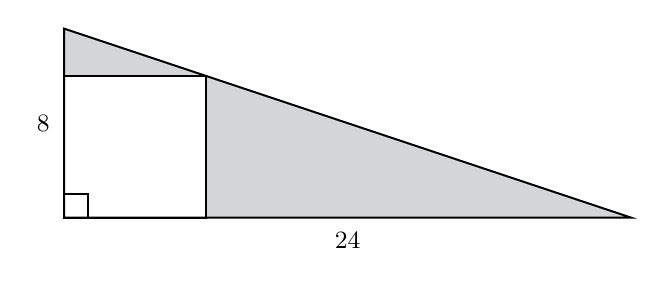
\begin{tikzpicture}[scale=0.3]
\coordinate (O) at (0,0); \coordinate (P) at (24,0); \coordinate (Q) at (0,8);
\fill[ink!20] (6,0)--(24,0)--(6,6)--cycle; \fill[ink!20] (0,6)--(6,6)--(0,8)--cycle;
\draw[line width=0.7pt] (O)--(P)--(Q)--cycle;
\draw[line width=0.7pt] (0,0) rectangle (6,6);
\draw[line width=0.5pt] (0,1)--(1,1)--(1,0);
\node[below,font=\small] at (12,-0.2) {24}; \node[left,font=\small] at (-0.2,4) {8};
\end{tikzpicture}}\gridbox
\vfill

\noindent\pnum{22} In the $xy$-plane, the line $y=kx-5$ has exactly one point in common with the parabola $y=x^2+3x+4$. What is the product of all possible values of $k$?\par\vspace{2.2mm}
\hspace*{7mm}(A)\ $-27$\\[1.8mm]
\hspace*{7mm}(B)\ $-3$\\[1.8mm]
\hspace*{7mm}(C)\ $9$\\[1.8mm]
\hspace*{7mm}(D)\ $27$
\vfill}}
\end{textblock*}
\clearpage

\end{document}
